\trilingualchapter{Theme Hotels with Functional Rooms: Beyond Decoration}{功能性主题酒店:超越装饰}{Themenhotels mit funktionalen Räumen: Über Dekoration hinaus}{}

Building on the Hyper Restaurant concept, Sue and Owen envisioned an even more ambitious project: a theme hotel where each room is not just decoratively themed, but functionally designed for specific activities. This chapter explores the concept of 主题酒店 (theme hotels | Themenhotels) with functional rooms that serve as activity spaces, integrated with social matching and hospitality services.

在超餐厅概念的基础上,Sue 和 Owen 设想了一个更加雄心勃勃的项目:一个主题酒店,其中每个房间不仅具有装饰性主题,而且为特定活动进行功能性设计。本章探讨功能性主题酒店(主题酒店)的概念,这些功能性房间作为活动空间,与社交匹配和酒店服务相结合。

Aufbauend auf dem Hyper-Restaurant-Konzept entwickelten Sue und Owen ein noch ehrgeizigeres Projekt: ein Themenhotel, in dem jeder Raum nicht nur dekorativ thematisiert ist, sondern funktional für spezifische Aktivitäten gestaltet ist. Dieses Kapitel erkundet das Konzept der Themenhotels (主题酒店) mit funktionalen Räumen, die als Aktivitätsräume dienen und mit sozialem Matching und Gastronomiedienstleistungen integriert sind.

\section{The Functional Theme Hotel Concept | 功能性主题酒店概念 | Das Konzept des funktionalen Themenhotels}

Unlike traditional theme hotels that focus primarily on decorative themes, the functional theme hotel creates spaces where the theme determines the room's purpose and capabilities.

\subsection{Core Philosophy}

\begin{itemize}
    \item \textbf{Function over form}: Theme serves a purpose, not just aesthetics
    \item \textbf{Activity-based design}: Rooms designed for specific activities
    \item \textbf{Social integration}: Spaces facilitate interaction and connection
    \item \textbf{Multi-purpose flexibility}: Rooms adapt to different needs
    \item \textbf{Technology integration}: Smart rooms enhance experiences
    \item \textbf{Wellness focus}: Health and well-being integrated throughout
\end{itemize}

\section{Functional Room Types | 功能性房间类型 | Funktionale Raumtypen}

\begin{figure}[h]
\centering
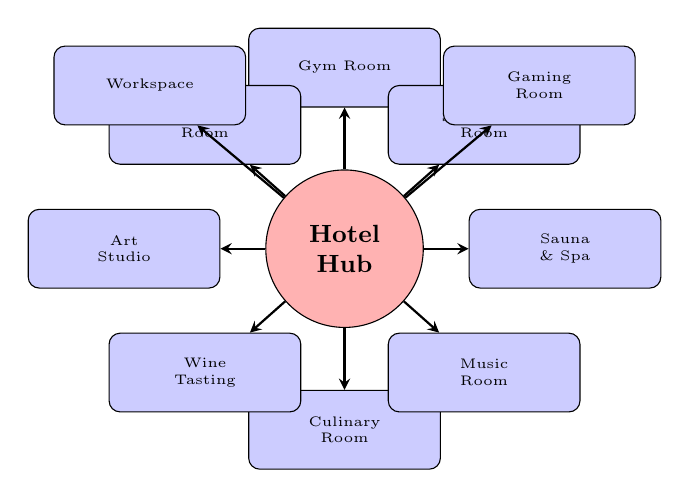
\begin{tikzpicture}[
    node distance=1.8cm,
    auto,
    room/.style={rectangle, draw, fill=blue!20, text width=2.2cm, text centered, rounded corners, minimum height=1cm, font=\tiny},
    central/.style={circle, draw, fill=red!30, text width=1.5cm, text centered, minimum size=2cm, font=\small\bfseries},
    arrow/.style={thick,->,>=stealth}
]
    % Central hub
    \node [central] (hub) {Hotel\\Hub};
    
    % Fitness rooms
    \node [room, above of=hub, yshift=0.5cm] (gym) {Gym Room};
    \node [room, above left of=hub, xshift=-0.5cm, yshift=0.3cm] (yoga) {Yoga\\Room};
    \node [room, above right of=hub, xshift=0.5cm, yshift=0.3cm] (swim) {Swimming\\Room};
    
    % Wellness rooms
    \node [room, right of=hub, xshift=1cm] (sauna) {Sauna\\\& Spa};
    
    % Culinary rooms
    \node [room, below of=hub, yshift=-0.5cm] (culinary) {Culinary\\Room};
    \node [room, below left of=hub, xshift=-0.5cm, yshift=-0.3cm] (wine) {Wine\\Tasting};
    
    % Creative rooms
    \node [room, left of=hub, xshift=-1cm] (art) {Art\\Studio};
    \node [room, below right of=hub, xshift=0.5cm, yshift=-0.3cm] (music) {Music\\Room};
    
    % Business rooms
    \node [room, above left of=hub, xshift=-1.2cm, yshift=0.8cm] (work) {Workspace};
    \node [room, above right of=hub, xshift=1.2cm, yshift=0.8cm] (gaming) {Gaming\\Room};
    
    % Arrows
    \draw [arrow] (hub) -- (gym);
    \draw [arrow] (hub) -- (yoga);
    \draw [arrow] (hub) -- (swim);
    \draw [arrow] (hub) -- (sauna);
    \draw [arrow] (hub) -- (culinary);
    \draw [arrow] (hub) -- (wine);
    \draw [arrow] (hub) -- (art);
    \draw [arrow] (hub) -- (music);
    \draw [arrow] (hub) -- (work);
    \draw [arrow] (hub) -- (gaming);
\end{tikzpicture}
\caption{Functional Theme Hotel Room Types}
\label{fig:theme_hotel_rooms}
\end{figure}

\subsection{Fitness and Wellness Rooms}

\subsubsection{Gym Room}

\begin{itemize}
    \item \textbf{Equipment}: Full gym setup (treadmills, weights, machines)
    \item \textbf{Virtual training}: Interactive screens with workout programs
    \item \textbf{Personal trainers}: Available for booking
    \item \textbf{Group classes}: Scheduled fitness sessions
    \item \textbf{Social matching}: Pair guests with similar fitness goals
    \item \textbf{Progress tracking}: Integration with fitness apps
\end{itemize}

\subsubsection{Yoga and Meditation Room}

\begin{itemize}
    \item \textbf{Design}: Peaceful, zen-like atmosphere
    \item \textbf{Equipment}: Mats, blocks, bolsters, meditation cushions
    \item \textbf{Classes}: Scheduled yoga and meditation sessions
    \item \textbf{Technology}: Guided meditation apps, ambient sound systems
    \item \textbf{Group sessions}: Social meditation experiences
    \item \textbf{Private sessions}: Individual or couple bookings
\end{itemize}

\subsubsection{Swimming Room}

\begin{itemize}
    \item \textbf{Pool design}: Indoor pool with various depths
    \item \textbf{Aquatic fitness}: Water aerobics, swimming lessons
    \item \textbf{Recreation}: Leisure swimming, pool games
    \item \textbf{Social activities}: Pool parties, group swim sessions
    \item \textbf{Safety}: Lifeguard services, safety equipment
    \item \textbf{Amenities}: Changing rooms, towels, poolside service
\end{itemize}

\subsubsection{Sauna and Spa Room}

\begin{itemize}
    \item \textbf{Sauna facilities}: Traditional and infrared saunas
    \item \textbf{Steam rooms}: Relaxation and detoxification
    \item \textbf{Cold plunge}: Contrast therapy
    \item \textbf{Relaxation areas}: Quiet spaces for post-sauna rest
    \item \textbf{Spa services}: Massage, facials (by appointment)
    \item \textbf{Social matching}: Wellness-focused connections
\end{itemize}

\subsection{Culinary Experience Rooms | 烹饪体验房间 | Kulinarische Erlebnisräume}

\subsubsection{Culinary Room}

\begin{itemize}
    \item \textbf{Full kitchen}: Professional-grade equipment
    \item \textbf{Cooking classes}: Hands-on culinary education
    \item \textbf{Group cooking}: Collaborative meal preparation
    \item \textbf{Chef experiences}: Private chef services
    \item \textbf{Social dining}: Cook and eat together experiences
    \item \textbf{Competition cooking}: Culinary challenges and games
\end{itemize}

\subsubsection{Wine and Tasting Room}

\begin{itemize}
    \item \textbf{Tasting setup}: Proper glassware, spittoons, tasting notes
    \item \textbf{Wine education}: Classes and seminars
    \item \textbf{Pairing experiences}: Food and wine matching
    \item \textbf{Social tastings}: Group tasting events
    \item \textbf{Storage}: Wine storage for guests
    \item \textbf{Expert sommeliers}: Available for guidance
\end{itemize}

\subsection{Creative and Entertainment Rooms | 创意与娱乐房间 | Kreative und Unterhaltungsräume}

\subsubsection{Art Studio}

\begin{itemize}
    \item \textbf{Supplies}: Various art materials and tools
    \item \textbf{Workspace}: Easels, tables, storage
    \item \textbf{Classes}: Art workshops and lessons
    \item \textbf{Social art}: Group art projects
    \item \textbf{Exhibition space}: Display guest creations
    \item \textbf{Instructors}: Professional artists available
\end{itemize}

\subsubsection{Music Room}

\begin{itemize}
    \item \textbf{Instruments}: Various instruments available
    \item \textbf{Recording equipment}: Basic studio setup
    \item \textbf{Practice space}: Soundproofed for practice
    \item \textbf{Group sessions}: Jam sessions, music classes
    \item \textbf{Performances}: Small concerts and recitals
    \item \textbf{Social matching}: Connect musicians
\end{itemize}

\subsubsection{Gaming Room}

\begin{itemize}
    \item \textbf{Video games}: Consoles, VR equipment
    \item \textbf{Board games}: Extensive collection
    \item \textbf{Competitive gaming}: Tournaments and competitions
    \item \textbf{Social gaming}: Multiplayer experiences
    \item \textbf{Streaming setup}: For content creators
    \item \textbf{Esports events}: Organized competitions
\end{itemize}

\subsection{Business and Learning Rooms | 商务与学习房间 | Geschäfts- und Lernräume}

\subsubsection{Workspace Room}

\begin{itemize}
    \item \textbf{Office setup}: Desks, ergonomic chairs, monitors
    \item \textbf{Meeting space}: Conference table, presentation equipment
    \item \textbf{Technology}: High-speed internet, printing, video conferencing
    \item \textbf{Coworking}: Shared workspace environment
    \item \textbf{Networking}: Facilitated business connections
    \item \textbf{Quiet zones}: Focused work areas
\end{itemize}

\subsubsection{Library and Study Room}

\begin{itemize}
    \item \textbf{Book collection}: Curated selection
    \item \textbf{Reading spaces}: Comfortable seating, good lighting
    \item \textbf{Study areas}: Quiet, focused environments
    \item \textbf{Book clubs}: Social reading groups
    \item \textbf{Author events}: Readings and discussions
    \item \textbf{Digital resources}: E-books, online databases
\end{itemize}

\section{Social Matching Integration | 社交匹配整合 | Soziale Matching-Integration}

\subsection{Matching by Interest | 按兴趣匹配 | Matching nach Interesse}

\begin{itemize}
    \item \textbf{Activity preferences}: Match guests with similar interests
    \item \textbf{Skill levels}: Pair beginners with experienced guests
    \item \textbf{Social goals}: Connect those seeking friendship, networking, or romance
    \item \textbf{Group formation}: Create activity groups automatically
    \item \textbf{Event matching}: Match guests to scheduled activities
\end{itemize}

\subsection{Technology Platform | 技术平台 | Technologieplattform}

\subsubsection{Mobile App Features}

\begin{itemize}
    \item \textbf{Profile creation}: Interests, skills, social preferences
    \item \textbf{Activity booking}: Reserve functional rooms
    \item \textbf{Social matching}: See compatible guests
    \item \textbf{Event discovery}: Find activities and events
    \item \textbf{Messaging}: Communicate with matches (with consent)
    \item \textbf{Activity tracking}: Record participation and achievements
\end{itemize}

\subsubsection{In-Hotel Technology}

\begin{itemize}
    \item \textbf{Room displays}: Show available activities and matches
    \item \textbf{Smart room controls}: Adjust environment for activities
    \item \textbf{Wearable integration}: Track fitness, activities
    \item \textbf{Digital concierge}: AI-assisted recommendations
    \item \textbf{Social boards}: Display group activities and opportunities
\end{itemize}

\section{Design and Architecture | 设计与建筑 | Design und Architektur}

\subsection{Room Design Principles | 房间设计原则 | Raumdesignprinzipien}

\subsubsection{Functionality First}

\begin{itemize}
    \item Design supports the room's primary function
    \item Equipment and tools are accessible and high-quality
    \item Safety considerations are paramount
    \item Flexibility for different use cases
    \item Technology seamlessly integrated
\end{itemize}

\subsubsection{Aesthetic Integration}

\begin{itemize}
    \item Theme enhances function, doesn't distract
    \item Comfortable and inviting atmosphere
    \item Professional yet approachable
    \item Clean and well-maintained
    \item Inspiring and motivating
\end{itemize}

\subsection{Common Areas | 公共区域 | Gemeinschaftsbereiche}

\begin{itemize}
    \item \textbf{Lobby}: Social hub with activity displays
    \item \textbf{Restaurant}: Hyper Restaurant concept integrated
    \item \textbf{Lounges}: Casual social spaces
    \item \textbf{Outdoor spaces}: Gardens, terraces, patios
    \item \textbf{Event spaces}: For larger gatherings
\end{itemize}

\section{Operational Model | 运营模式 | Betriebsmodell}

\subsection{Booking System | 预订系统 | Buchungssystem}

\begin{itemize}
    \item \textbf{Room reservations}: Book functional rooms by activity
    \item \textbf{Time slots}: Hourly or session-based booking
    \item \textbf{Group bookings}: Reserve for social groups
    \item \textbf{Private sessions}: Individual or couple bookings
    \item \textbf{Event participation}: Sign up for scheduled activities
\end{itemize}

\subsection{Staffing | 人员配置 | Personalwesen}

\subsubsection{Specialized Staff}

\begin{itemize}
    \item \textbf{Activity coordinators}: Manage each room type
    \item \textbf{Instructors}: Fitness, culinary, art, music experts
    \item \textbf{Social facilitators}: Help with matching and connections
    \item \textbf{Technology support}: Assist with apps and systems
    \item \textbf{Concierge}: Activity recommendations and bookings
\end{itemize}

\subsubsection{Training}

\begin{itemize}
    \item Activity-specific expertise
    \item Social facilitation skills
    \item Safety and first aid
    \item Technology proficiency
    \item Customer service excellence
\end{itemize}

\subsection{Pricing Models | 定价模式 | Preismodelle}

\subsubsection{Accommodation Packages}

\begin{itemize}
    \item \textbf{Basic}: Standard room, limited activity access
    \item \textbf{Activity package}: Includes specific room access
    \item \textbf{All-access}: Unlimited functional room use
    \item \textbf{Premium}: Private sessions, personal trainers, exclusive events
\end{itemize}

\subsubsection{Activity Fees}

\begin{itemize}
    \item Some activities included in room rate
    \item Premium activities require additional fees
    \item Group discounts for social activities
    \item Membership tiers for frequent guests
\end{itemize}

\section{Integration with Hyper Restaurant | 与超餐厅的整合 | Integration mit Hyper-Restaurant}

\subsection{Seamless Experience | 无缝体验 | Nahtloses Erlebnis}

\begin{itemize}
    \item Culinary room connects to restaurant
    \item Cooking classes lead to dining experiences
    \item Social matching works across hotel and restaurant
    \item Shared gamification platform
    \item Unified loyalty program
\end{itemize}

\subsection{Cross-Promotion | 交叉推广 | Cross-Promotion}

\begin{itemize}
    \item Restaurant guests can access hotel activities
    \item Hotel guests receive restaurant benefits
    \item Combined packages and memberships
    \item Shared events and experiences
\end{itemize}

\section{Challenges and Solutions | 挑战与解决方案 | Herausforderungen und Lösungen}

\subsection{Common Challenges}

\begin{itemize}
    \item \textbf{Space requirements}: Functional rooms need significant space
    \item \textbf{Equipment costs}: High-quality equipment is expensive
    \item \textbf{Maintenance}: Complex facilities require ongoing care
    \item \textbf{Staff expertise}: Need specialists for each area
    \item \textbf{Social dynamics}: Managing guest interactions
    \item \textbf{Technology complexity}: Multiple systems to integrate
\end{itemize}

\subsection{Solutions}

\begin{itemize}
    \item Phased development: Start with most popular room types
    \item Equipment partnerships: Work with suppliers for better pricing
    \item Preventive maintenance programs
    \item Cross-training staff in multiple areas
    \item Clear policies and trained facilitators
    \item Integrated technology platform
\end{itemize}

\trilingualsection{Key Takeaways}{关键要点}{Wichtige Erkenntnisse}{}

\begin{itemize}
    \item Functional theme hotels create value through activities, not just decoration
    \item Each room type serves specific purposes and attracts different guests
    \item Social matching enhances the experience and creates community
    \item Technology enables seamless booking, matching, and experiences
    \item Integration with restaurant creates comprehensive hospitality experience
    \item Quality equipment and staff are essential investments
    \item Flexibility allows for adaptation to guest needs
    \item Safety and privacy must be carefully managed
\end{itemize}

The functional theme hotel represents a new paradigm in hospitality, where accommodation becomes a gateway to experiences, activities, and connections. For Sue and Owen, this concept offered the opportunity to create something truly unique—a place where guests don't just stay, but live, learn, connect, and grow.
